% =============================================================================
% 作品说明文档 · MeetAgent（会合助手）
% 中国高校计算机大赛 — 人工智能创意赛（鸿蒙赛道）
% 依据 resource/submit_template.pdf（组委会编制 2026.06）
%
% 编译（建议 XeLaTeX，在 resource/ 目录下执行）：
%   xelatex 01-作品说明文档-MeetAgent会合助手.tex
%   xelatex 01-作品说明文档-MeetAgent会合助手.tex
% 提交 PDF 命名：01-作品说明文档+参赛队伍名称.pdf
% =============================================================================
\documentclass[UTF8,a4paper,zihao=-4]{ctexart}

\usepackage[
  a4paper,
  top=2.5cm,
  bottom=2.5cm,
  left=3cm,
  right=3cm,
  headheight=14pt,
  headsep=0.6cm,
  footskip=1.2cm
]{geometry}

\usepackage{setspace}
\setstretch{1.0}

\usepackage{graphicx}
\graphicspath{{figures/}}
\usepackage{booktabs}
\usepackage{array}
\usepackage{tabularx}
\usepackage{enumitem}
\usepackage{caption}
\usepackage{subcaption}
\usepackage{float}
\usepackage{xcolor}
\usepackage{listings}
\usepackage{tikz}
\usetikzlibrary{arrows.meta,positioning,shapes.geometric,fit,calc}
\usepackage{fancyhdr}
\usepackage{hyperref}
\usepackage{amsmath}

\hypersetup{
  colorlinks=true,
  linkcolor=black,
  urlcolor=blue!50!black,
  citecolor=black,
  pdftitle={作品说明文档 · MeetAgent 会合助手},
  pdfauthor={李祥熙}
}

\ctexset{
  section/format       = \zihao{3}\bfseries\centering,
  subsection/format    = \zihao{4}\bfseries,
  subsubsection/format = \zihao{-4}\bfseries,
  paragraph/format     = \zihao{5}\bfseries,
  section/name         = {,},
  section/number       = \chinese{section},
  section/aftername    = {、},
}

\captionsetup{font=small, labelfont=bf, labelsep=quad}
\captionsetup[figure]{name=图}
\captionsetup[table]{name=表}

\setlist[itemize]{leftmargin=2em,itemsep=0.15em,topsep=0.3em}
\setlist[enumerate]{leftmargin=2em,itemsep=0.15em,topsep=0.3em}

\pagestyle{fancy}
\fancyhf{}
\fancyhead[C]{\zihao{5}\songti 作品说明文档 · MeetAgent（会合助手）}
\renewcommand{\headrulewidth}{0.4pt}
\fancyfoot[RO,LE]{\zihao{5}\thepage}

\lstset{
  basicstyle=\zihao{5}\ttfamily,
  breaklines=true,
  frame=single,
  columns=fullflexible,
  keepspaces=true,
  showstringspaces=false,
  aboveskip=0.6em,
  belowskip=0.6em
}

\definecolor{maBlue}{HTML}{0A84FF}
\definecolor{maGreen}{HTML}{34C759}
\definecolor{maDark}{HTML}{121620}
\definecolor{maGray}{HTML}{6B7280}
\definecolor{maSoft}{HTML}{EEF3FA}

\newcommand{\WorkTitle}{MeetAgent · 会合助手}
\newcommand{\TeamName}{为了看Miku演唱会特前来拿奖金}
\newcommand{\AuthorNames}{李祥熙}
\newcommand{\ContestTrack}{人工智能创意赛（鸿蒙赛道）}
\newcommand{\Slogan}{引擎算数智能体解释，一次锁定最优会合}

\begin{document}
\pagestyle{empty}

% =============================================================================
\begin{center}
  {\zihao{2}\bfseries 作品说明文档}\\[1.2em]
  {\zihao{2}\bfseries \WorkTitle}\\[0.8em]
  {\zihao{3}\bfseries \AuthorNames}\\[1.6em]
  {\zihao{4} 中国高校计算机大赛 · \ContestTrack}\\[0.4em]
  {\zihao{4} 队伍：\TeamName}\\[0.4em]
  {\zihao{5} 2026}
\end{center}

\vspace{1.0em}
\noindent\rule{\textwidth}{0.6pt}

\begin{abstract}
\noindent
{\zihao{5}
\textbf{摘要：}
MeetAgent（会合助手）是一款 HarmonyOS 智能会合规划应用，面向网约车接人、亲友接送、校园/园区接驳等高频场景。
针对“固定上车点 + 单侧导航”导致的双方空等与绕路，应用将\textbf{确定性路线拦截引擎}与\textbf{工具调用型 LLM Agent}结合：
由高德实时/估算路径与本地评分生成步行、骑行、公交与原地等待等候选；
智能体理解自然语言约束并解释取舍，\textbf{所有 ETA、距离与折线均来自工具与引擎}。
用户确认后锁定方案，支持分享与打开地图；无大模型密钥时仍可离线规划，保证演示与实战可用性。
}
\end{abstract}

\noindent\rule{\textwidth}{0.6pt}
\tableofcontents
\newpage
\pagestyle{fancy}
\setcounter{page}{1}

% =============================================================================
\section{创意描述}
% =============================================================================

\begin{center}
  {\zihao{3}\bfseries \Slogan}
\end{center}

\vspace{0.35em}
{\zihao{5}\songti
一句话概括核心创新点。
}

\vspace{0.5em}
\noindent{\zihao{5}
\textbf{场景一句话：}
司机已经在路上，乘客还能不能动一动，让双方更快会合？MeetAgent 在出发前把这件事算清楚、说清楚、锁住执行。
}

% =============================================================================
\section{设计稿与技术方案}
% =============================================================================

\subsection{典型使用场景（为什么需要）}

\begin{table}[H]
\centering
\zihao{5}
\begin{tabularx}{\textwidth}{>{\bfseries}p{2.4cm}X}
\toprule
场景 & 痛点与 MeetAgent 价值 \\
\midrule
网约车 / 网约顺风车接人 &
司机按导航直奔原上车点，乘客周围发生严重拥堵，在最后1千米浪费十几二十分钟；
若乘客步行或骑行 5 分钟到其余没有拥堵的路段会合，司机可少堵 10-20 分钟。
应用给出可解释的“乘客动一点 vs 原地等”对比，并一键分享给乘客。 \\
亲友机场 / 高铁接送 &
航班/车次到达时间弹性大，固定“出站口等”常造成长时间空等。
接车方可在出发前按实时路况锁定一个双方都能接受的会合点，减少电话来回改口。 \\
校园 / 园区 / 医院接驳 &
校门、院区入口与内部步行/骑行差异大；
乘客可公交或骑行到更合适的大门/路口，司机避免绕行禁行区域。 \\
弱网 / 演示 / 无 Key &
赛场或地下车库网络不稳时，可开启演示 Fixture 或纯估算路径，
仍能完成规划—锁定—分享闭环。 \\
\bottomrule
\end{tabularx}
\caption{核心实用场景与价值}
\label{tab:scenarios}
\end{table}

\subsection{产品定位与赛题契合}

MeetAgent 覆盖\textbf{应用}、\textbf{Agent}、\textbf{用户体验}：

\begin{itemize}
  \item \textbf{应用：}完整 HarmonyOS HAP——主页地图、普通规划、智能助手、设置、锁定会话。
  \item \textbf{Agent：}OpenAI 兼容工具循环；路线/候选/评分/regeo 归工具，LLM 只选方案并解释。
  \item \textbf{体验：}深色液态玻璃主题、搜索优先选点、结果页切换方案即更新路线。
\end{itemize}

\subsection{用户主路径}

图~\ref{fig:user-flow} 为从打开 App 到锁定分享的主路径；图~\ref{fig:ui-home}--\ref{fig:ui-locked} 为对应实机界面。

\begin{figure}[H]
\centering
\begin{tikzpicture}[
  font=\zihao{5}\songti,
  box/.style={draw=maBlue!70, rounded corners=3pt, align=center,
    inner sep=5pt, minimum width=2.45cm, minimum height=0.95cm, fill=maSoft},
  arr/.style={-{Latex}, thick, maDark!70}
]
  \node[box] (home) {主页实时地图\\搜索 / 点选};
  \node[box, right=0.5cm of home] (assign) {确认用途\\乘客或司机};
  \node[box, right=0.5cm of assign] (plan) {普通规划\\或智能助手};
  \node[box, below=0.7cm of plan] (engine) {Hybrid 路线\\+ 引擎评分};
  \node[box, left=0.5cm of engine] (cards) {多方案卡片\\切换路线};
  \node[box, left=0.5cm of cards] (lock) {确认锁定\\分享 / 导航};

  \draw[arr] (home) -- (assign);
  \draw[arr] (assign) -- (plan);
  \draw[arr] (plan) -- (engine);
  \draw[arr] (engine) -- (cards);
  \draw[arr] (cards) -- (lock);
\end{tikzpicture}
\caption{MeetAgent 用户主路径}
\label{fig:user-flow}
\end{figure}

\noindent\textbf{实操步骤：}
\begin{enumerate}
  \item 主页在高德底图上搜索或点选地点（可开路况）；
  \item 弹层确认用途（司机模式：\emph{我的乘客在这里} / \emph{我从这里出发}）；
  \item 地点以附近 POI 名称展示，写入草稿；
  \item \textbf{普通规划}调整乘客方式后优化，或\textbf{智能助手}用自然语言约束；
  \item 对比卡片、查看路线与会合 POI，确认锁定后分享或打开地图。
\end{enumerate}

\subsection{实机界面（设计稿）}

\begin{figure}[H]
  \centering
  \begin{subfigure}{0.48\textwidth}
    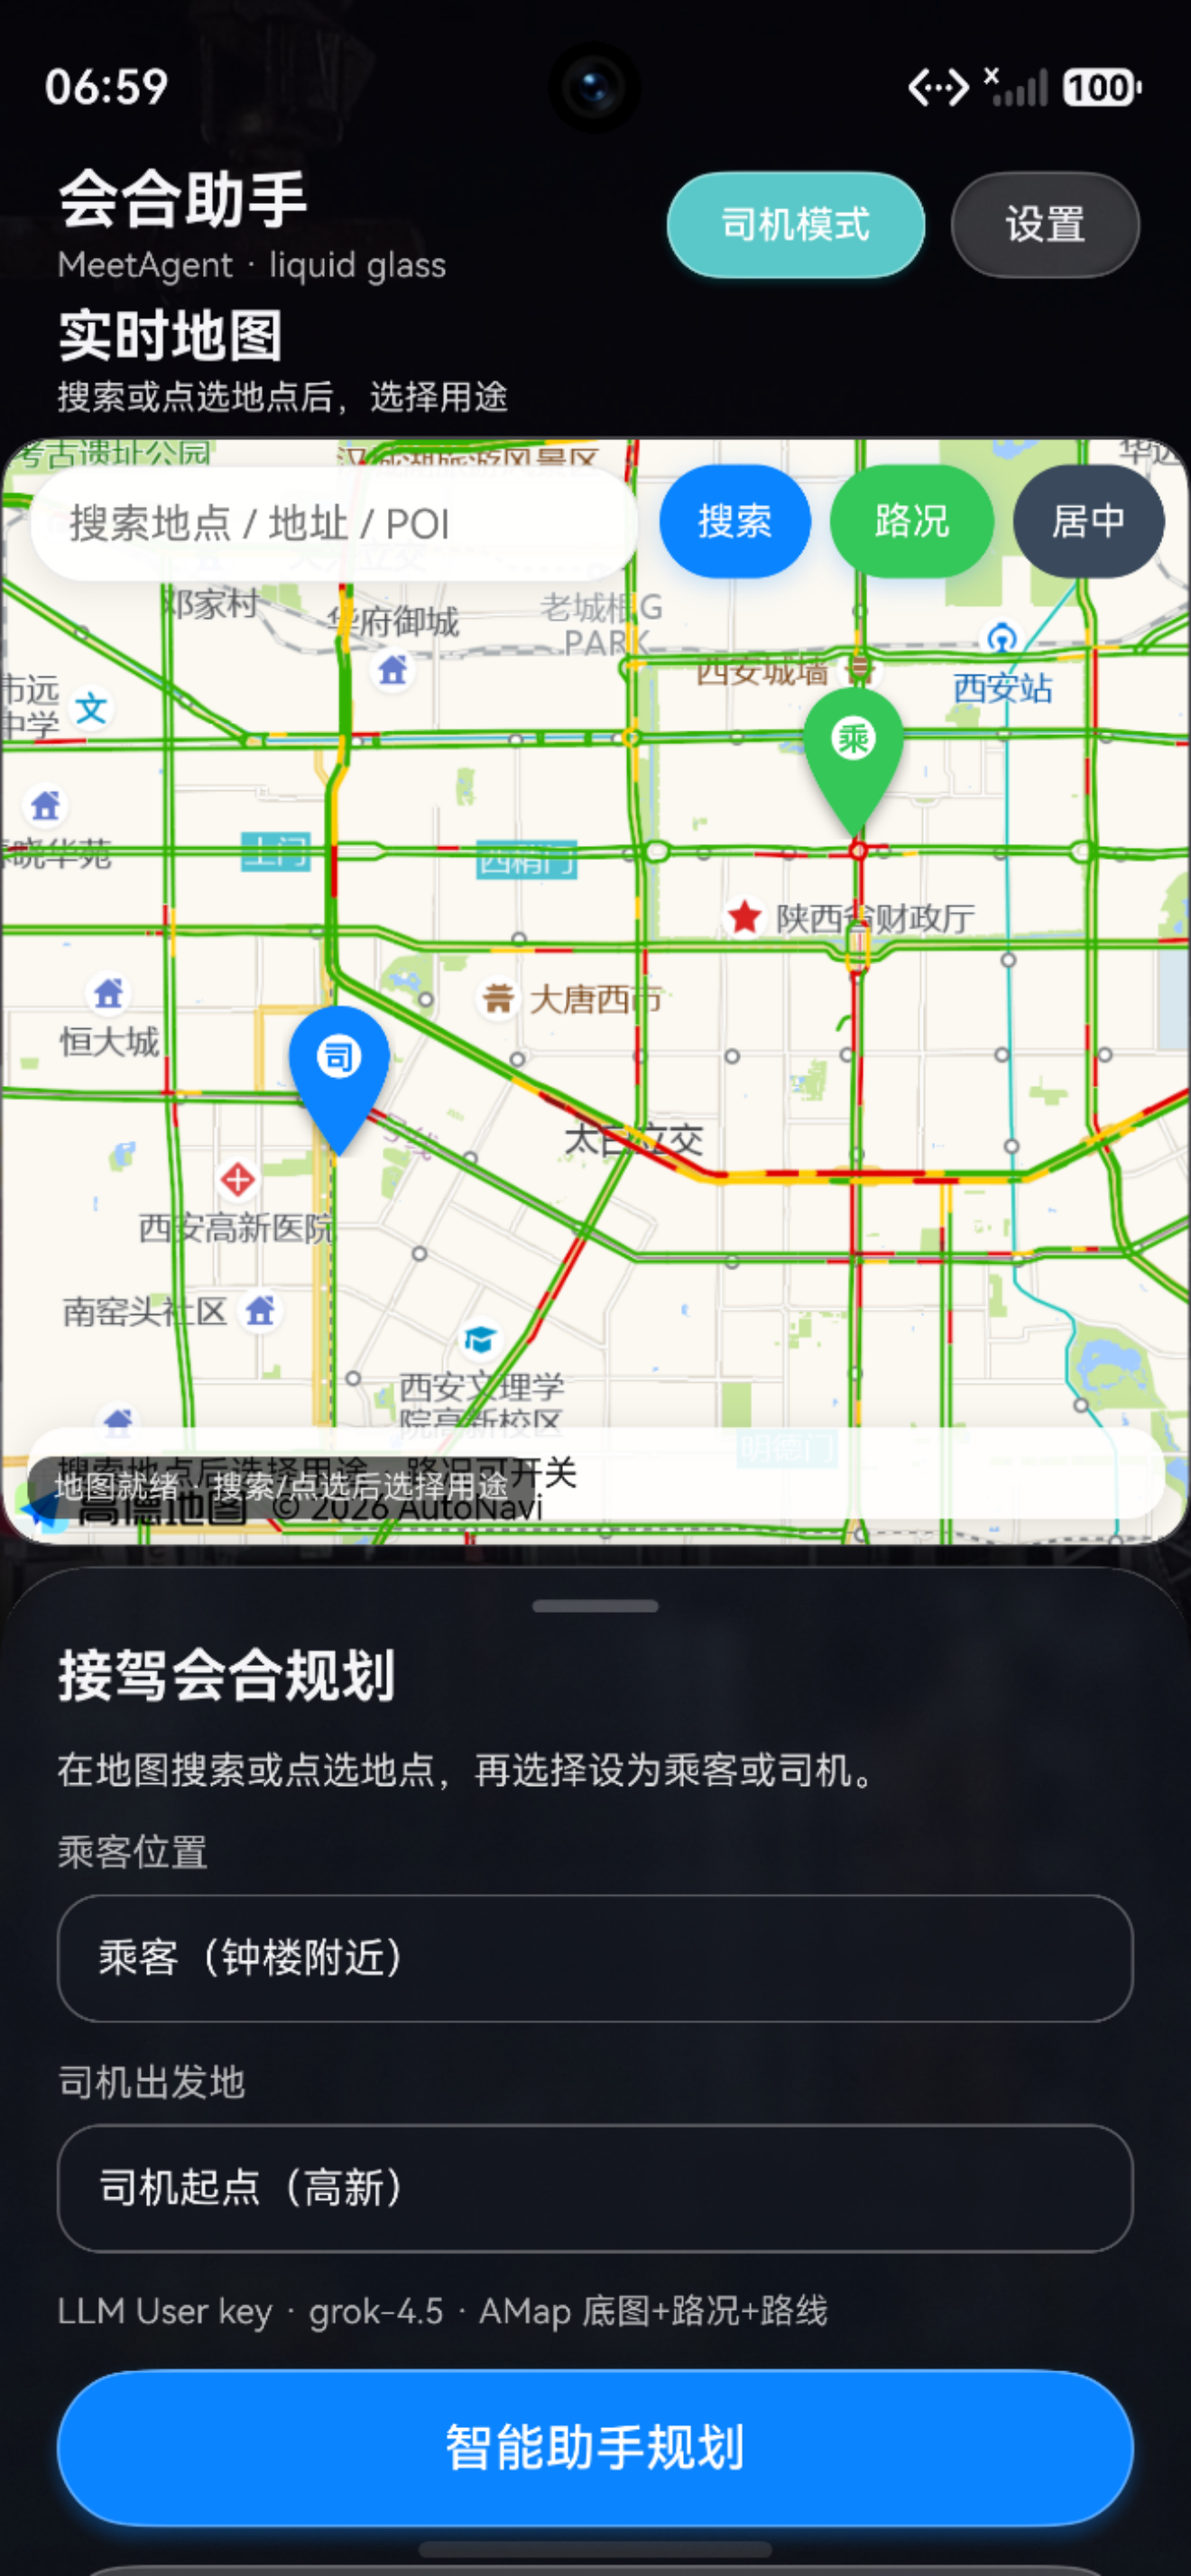
\includegraphics[width=\linewidth]{home.png}
    \caption{主页：实时底图、路况与司/乘标注}
    \label{fig:ui-home}
  \end{subfigure}\hfill
  \begin{subfigure}{0.48\textwidth}
    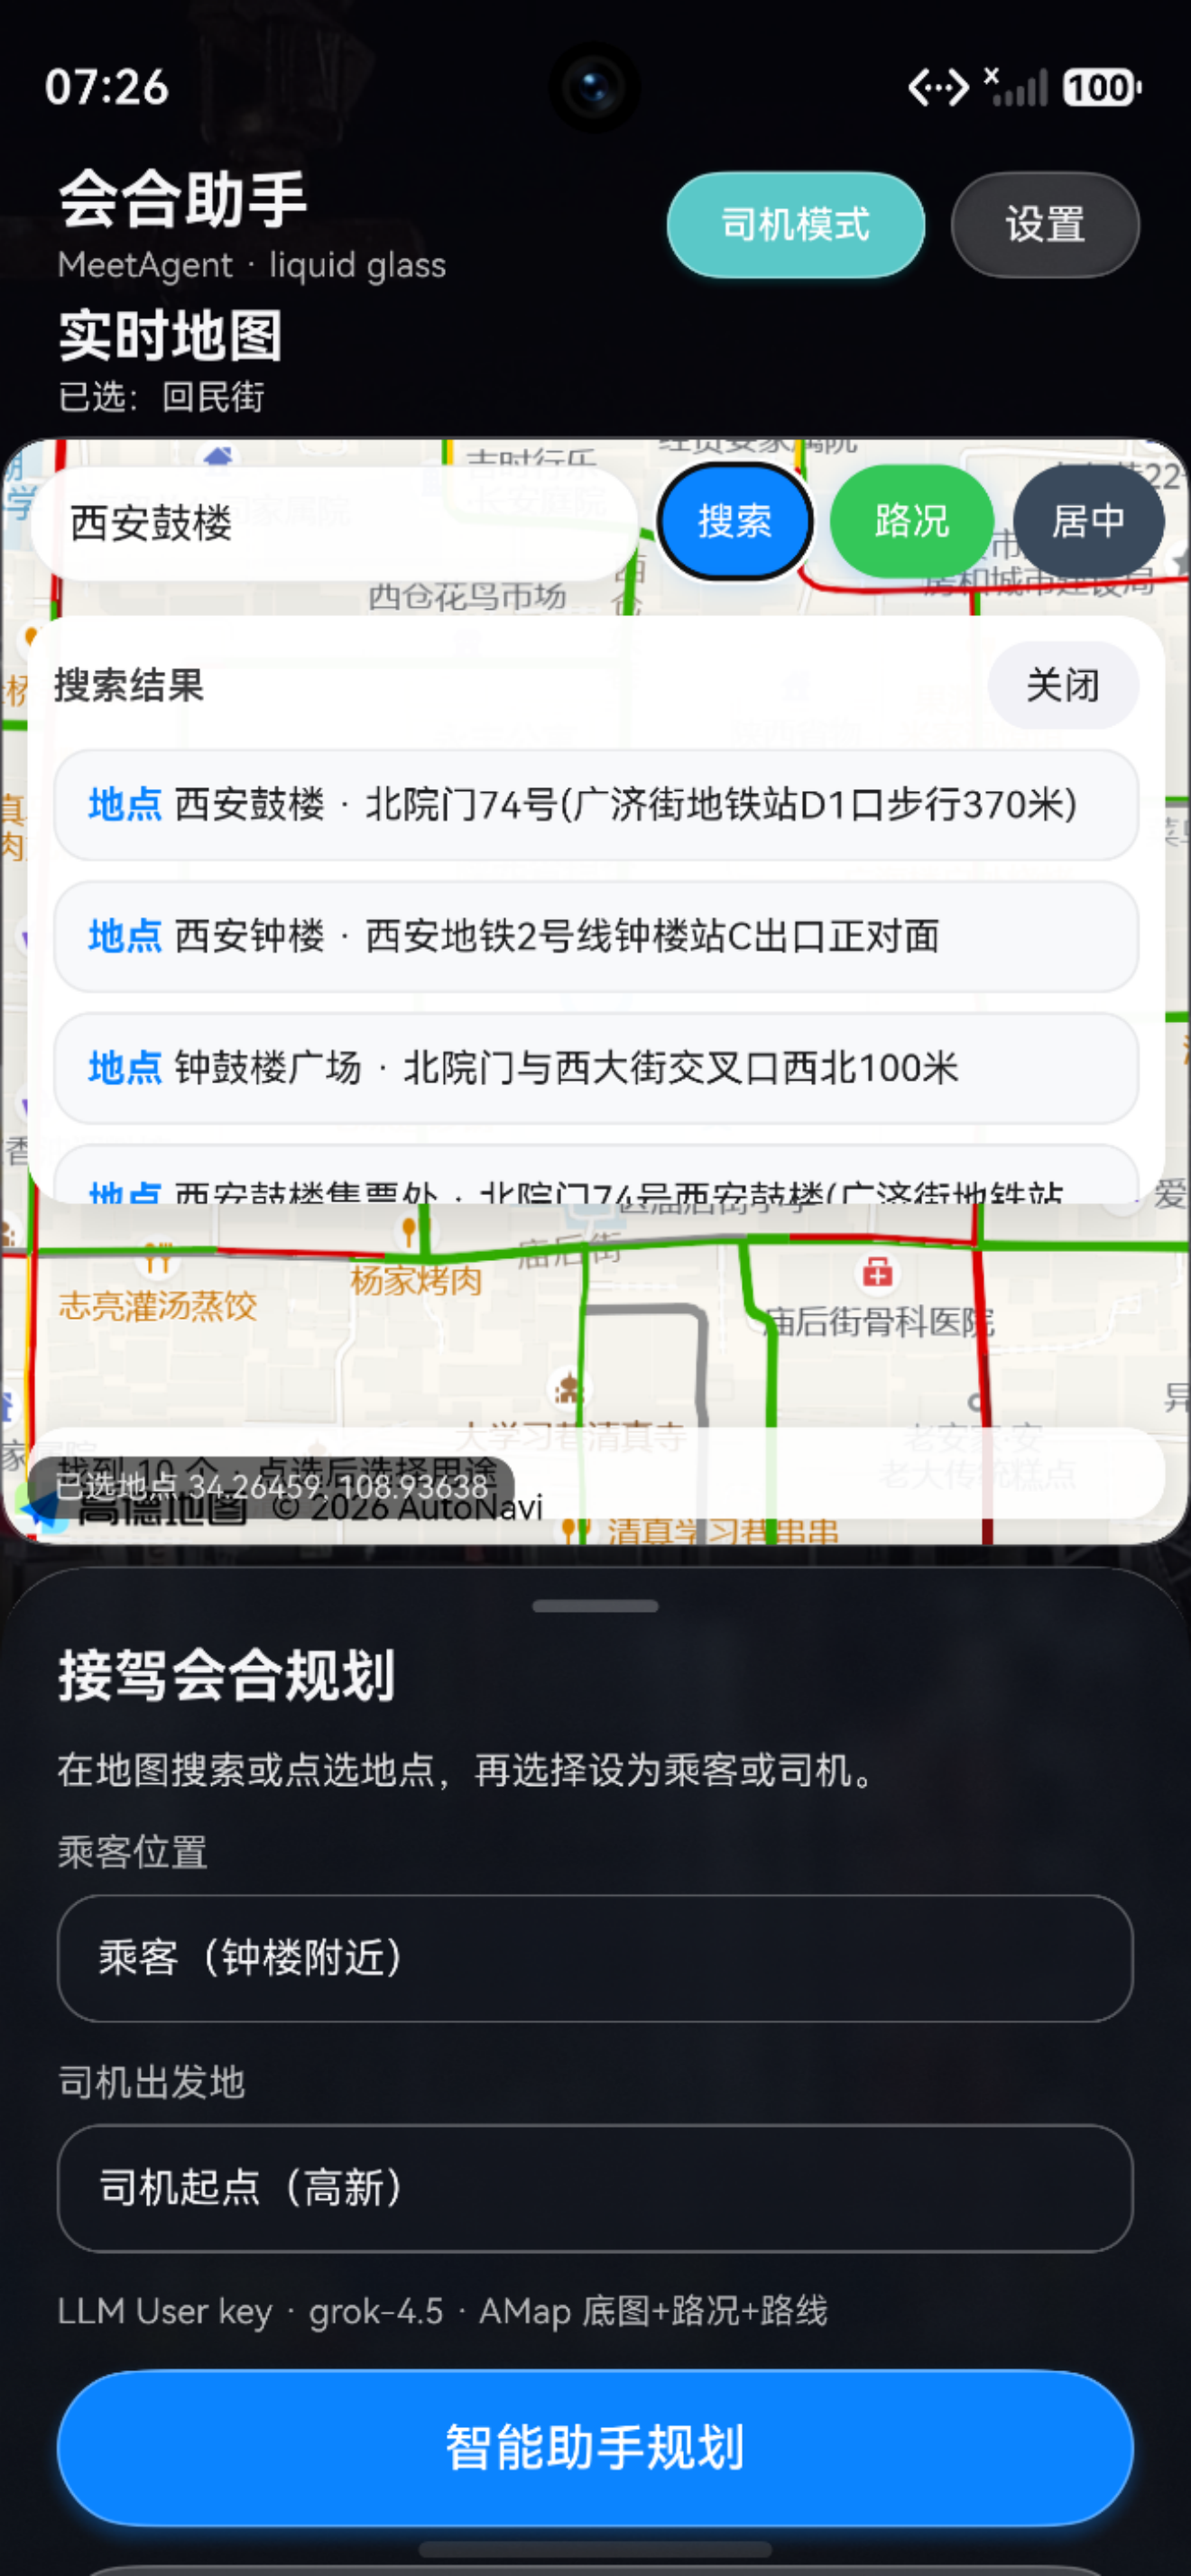
\includegraphics[width=\linewidth]{search.png}
    \caption{地点搜索}
    \label{fig:ui-search}
  \end{subfigure}
  \caption{主页地图与搜索}
\end{figure}

\begin{figure}[H]
  \centering
  \begin{subfigure}{0.48\textwidth}
    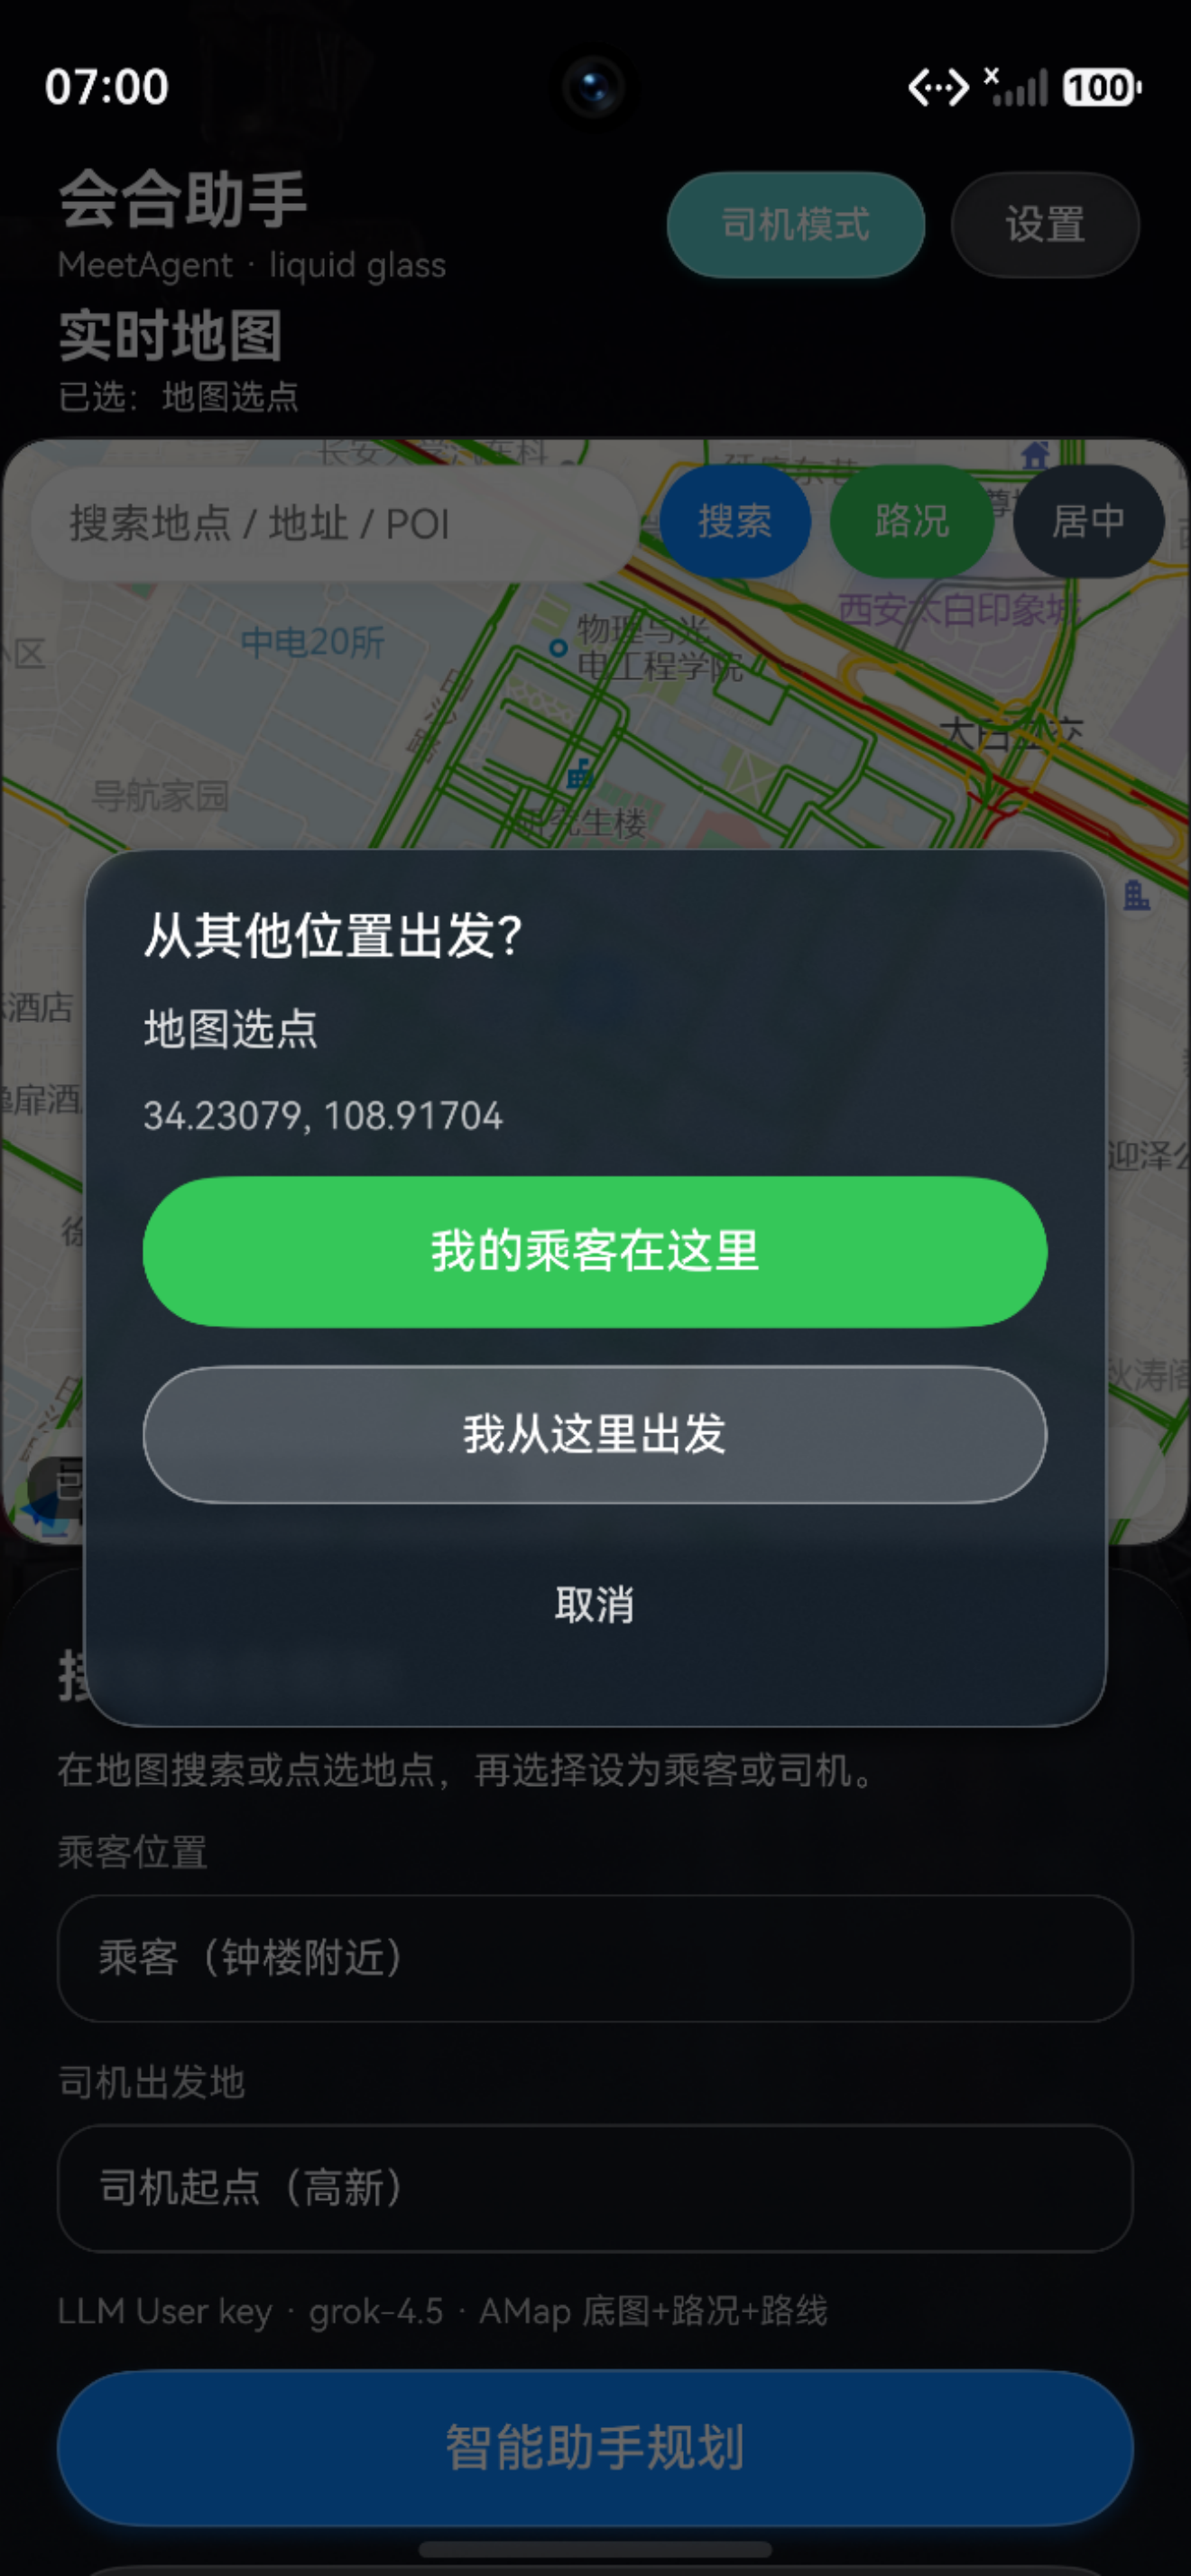
\includegraphics[width=\linewidth]{select_from_map.png}
    \caption{点选后确认用途（司机/乘客）}
    \label{fig:ui-select}
  \end{subfigure}\hfill
  \begin{subfigure}{0.48\textwidth}
    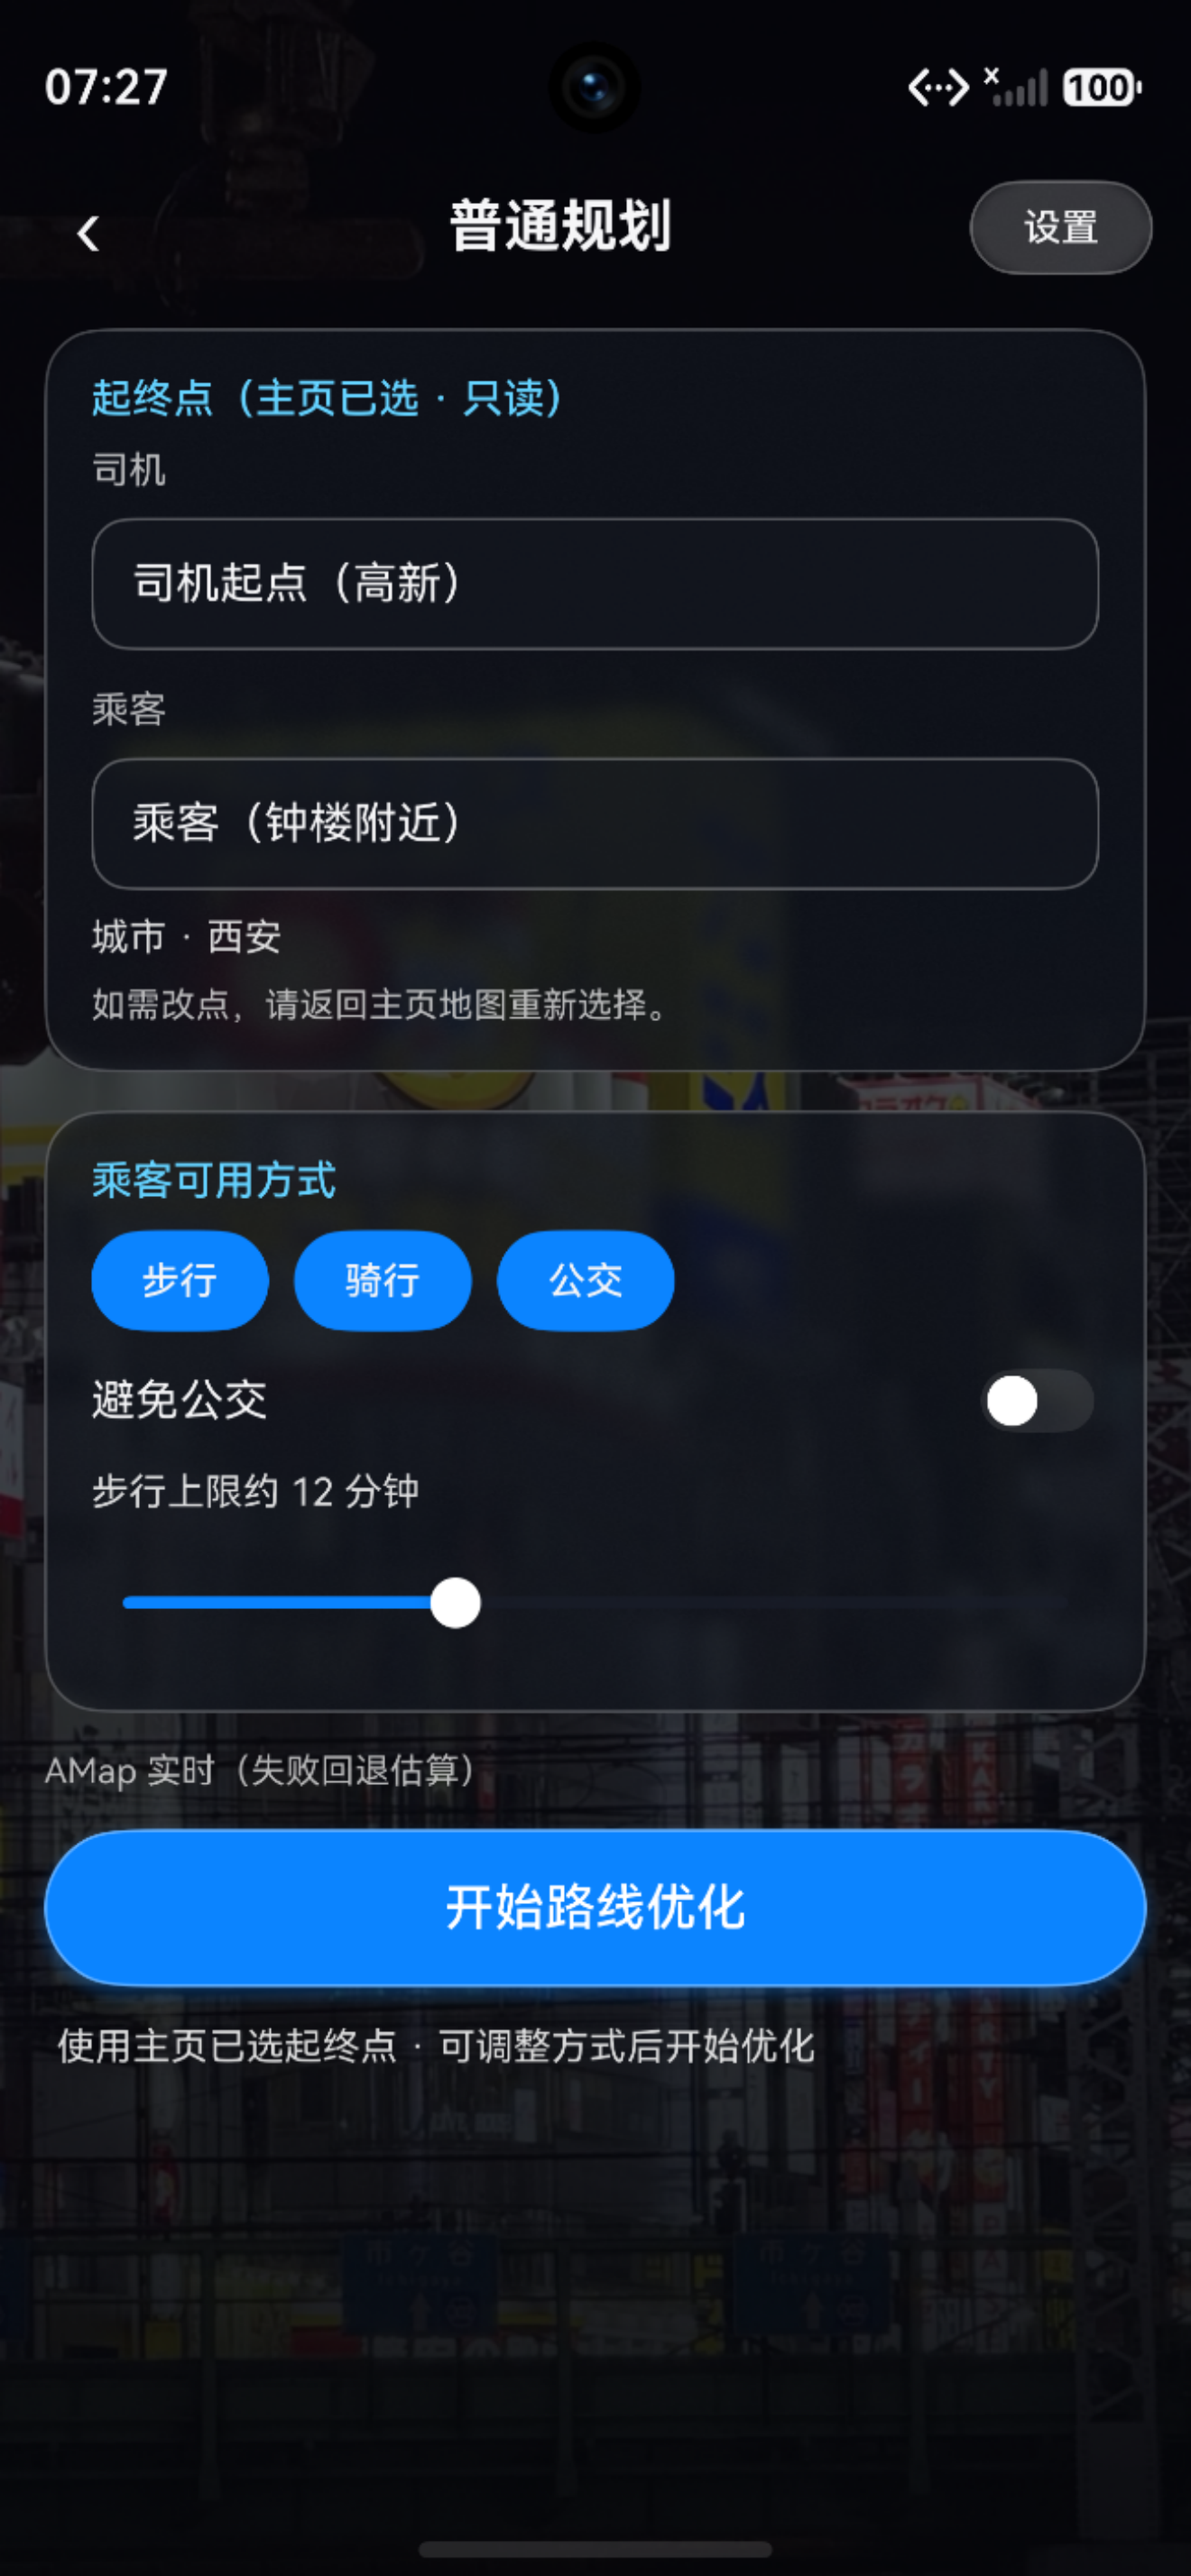
\includegraphics[width=\linewidth]{normal_planning.png}
    \caption{普通规划}
    \label{fig:ui-plan}
  \end{subfigure}
  \caption{选点确认与普通规划}
\end{figure}

\begin{figure}[H]
  \centering
  \begin{subfigure}{0.48\textwidth}
    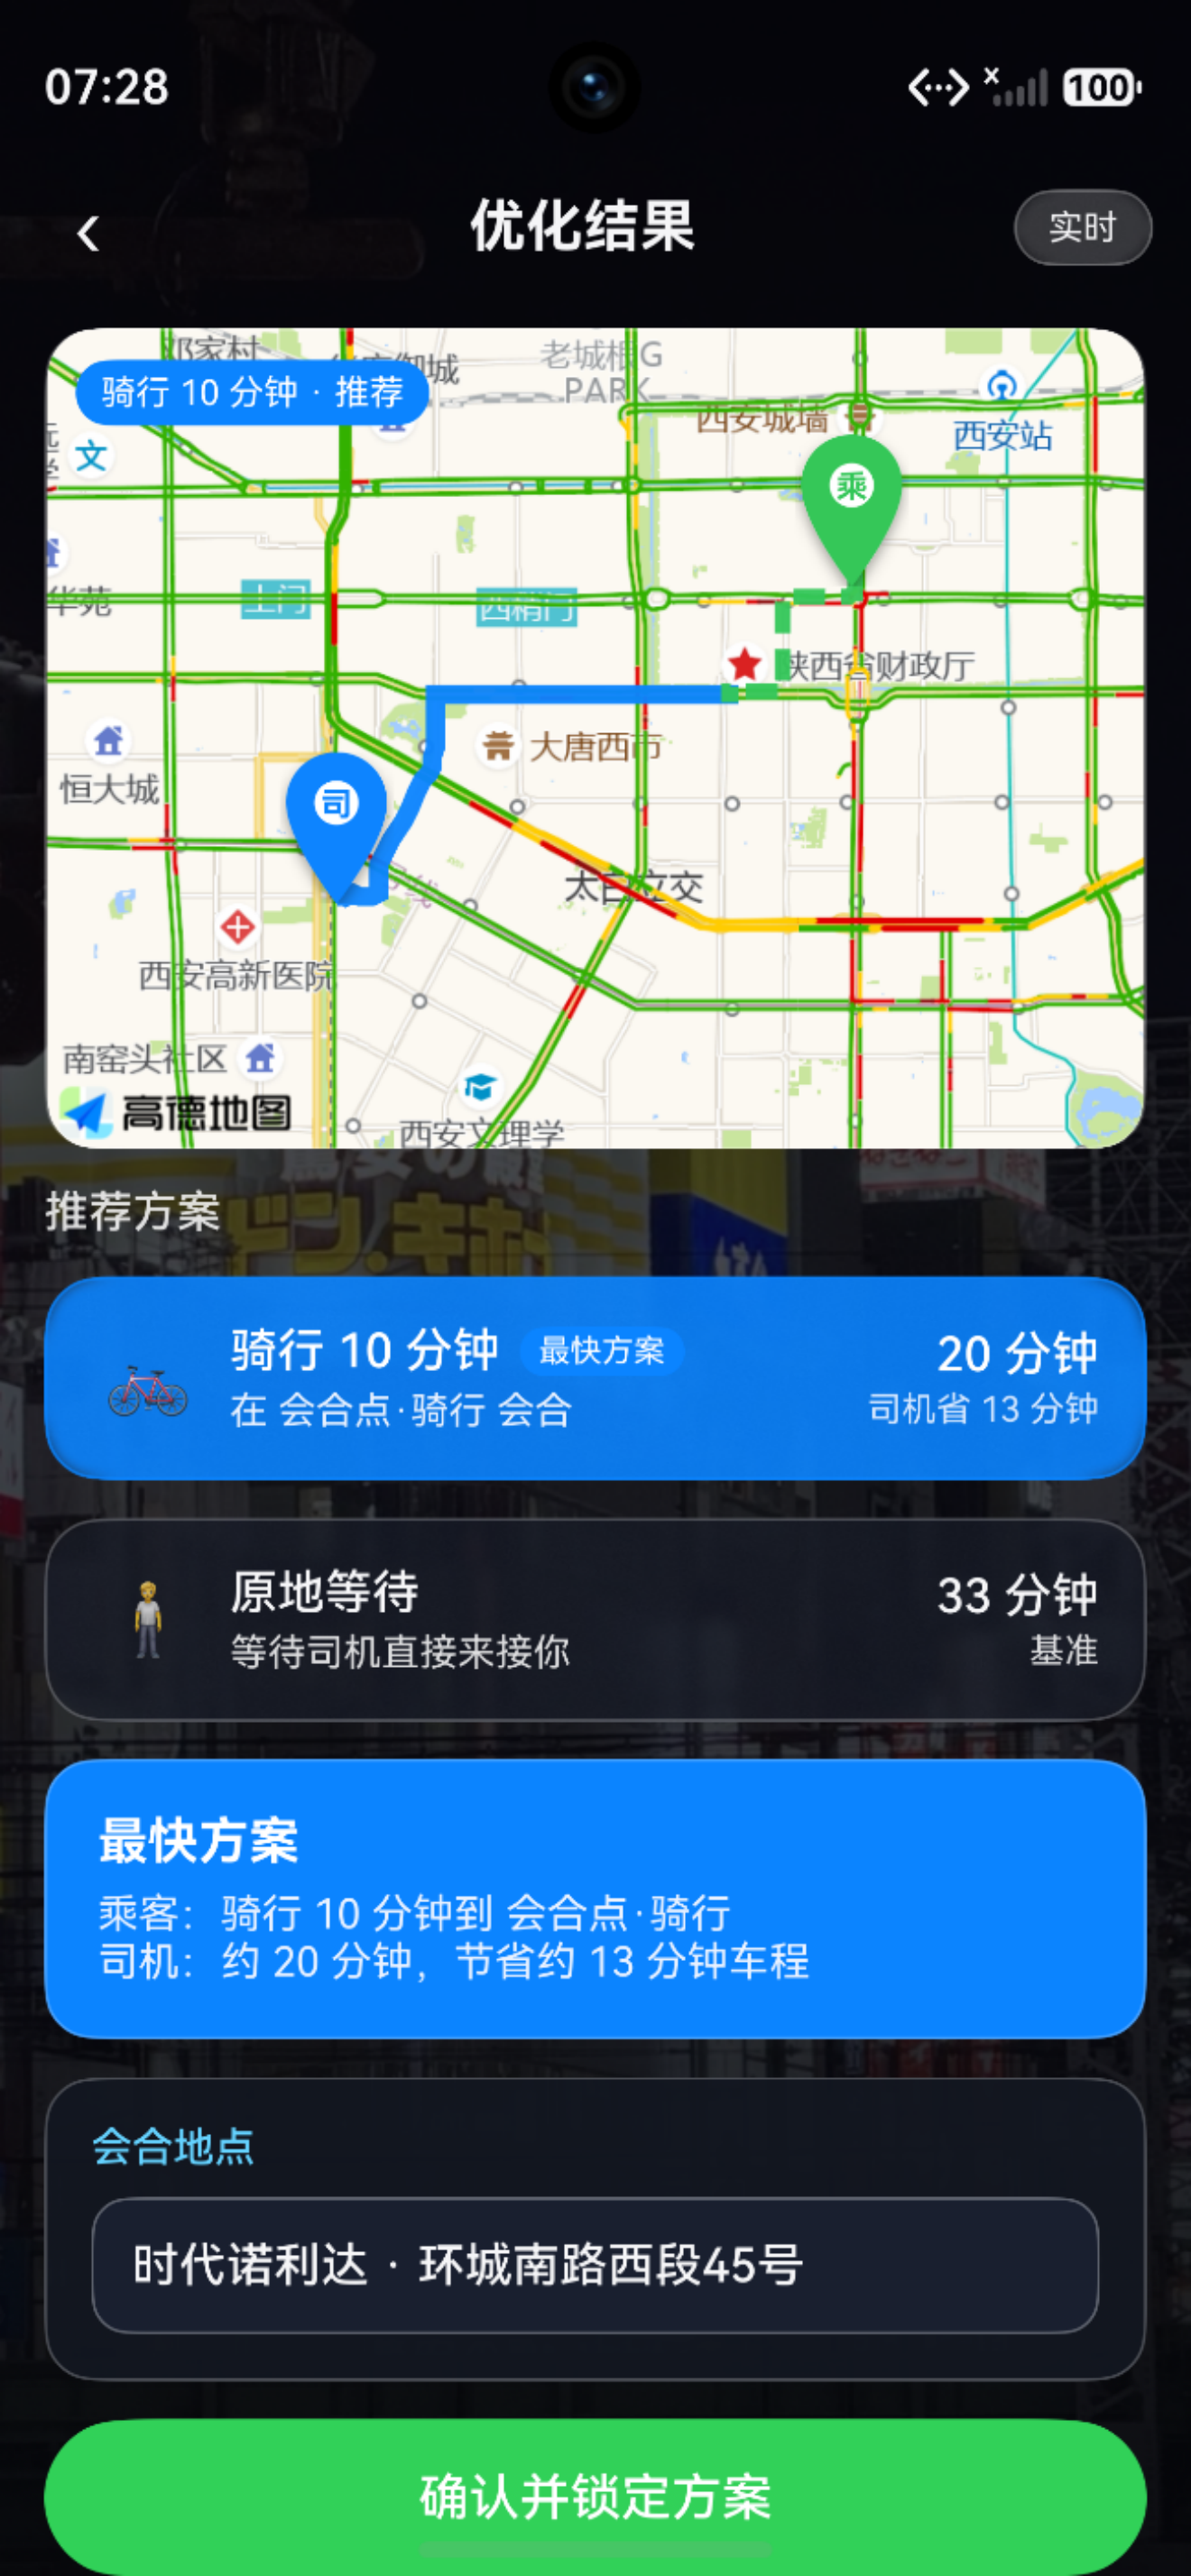
\includegraphics[width=\linewidth]{result_normal.png}
    \caption{普通规划结果：路线 + 方案卡片}
    \label{fig:ui-result-n}
  \end{subfigure}\hfill
  \begin{subfigure}{0.48\textwidth}
    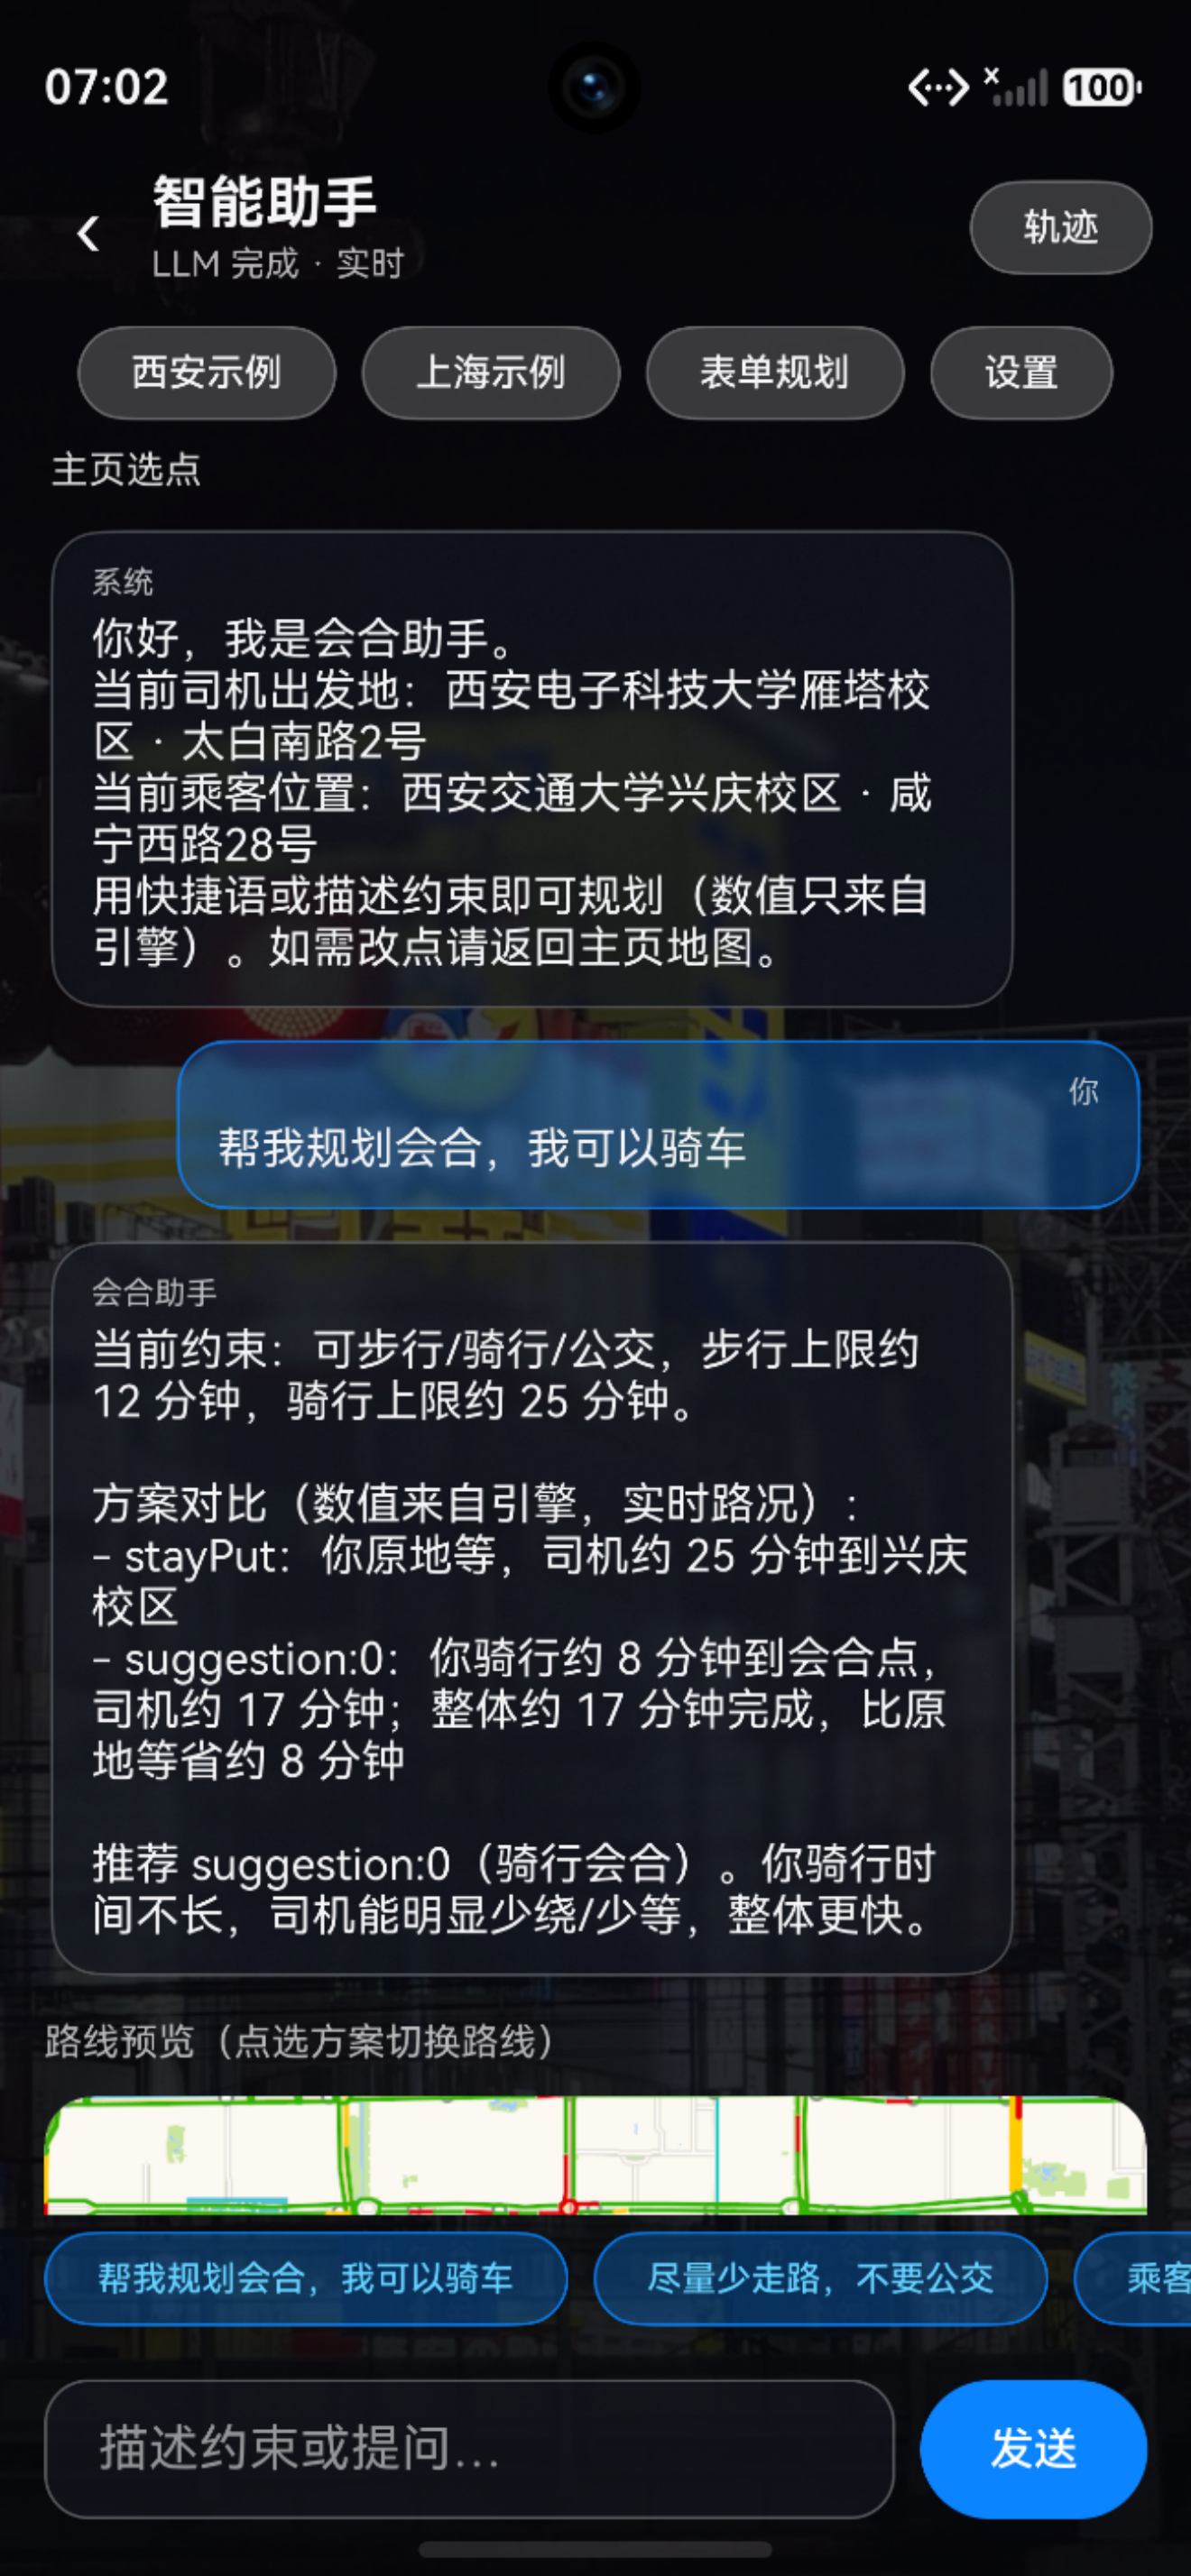
\includegraphics[width=\linewidth]{result_agent_1.png}
    \caption{智能助手：对话 + 路线预览}
    \label{fig:ui-agent1}
  \end{subfigure}
  \caption{规划结果与智能助手}
\end{figure}

\begin{figure}[H]
  \centering
  \begin{subfigure}{0.48\textwidth}
    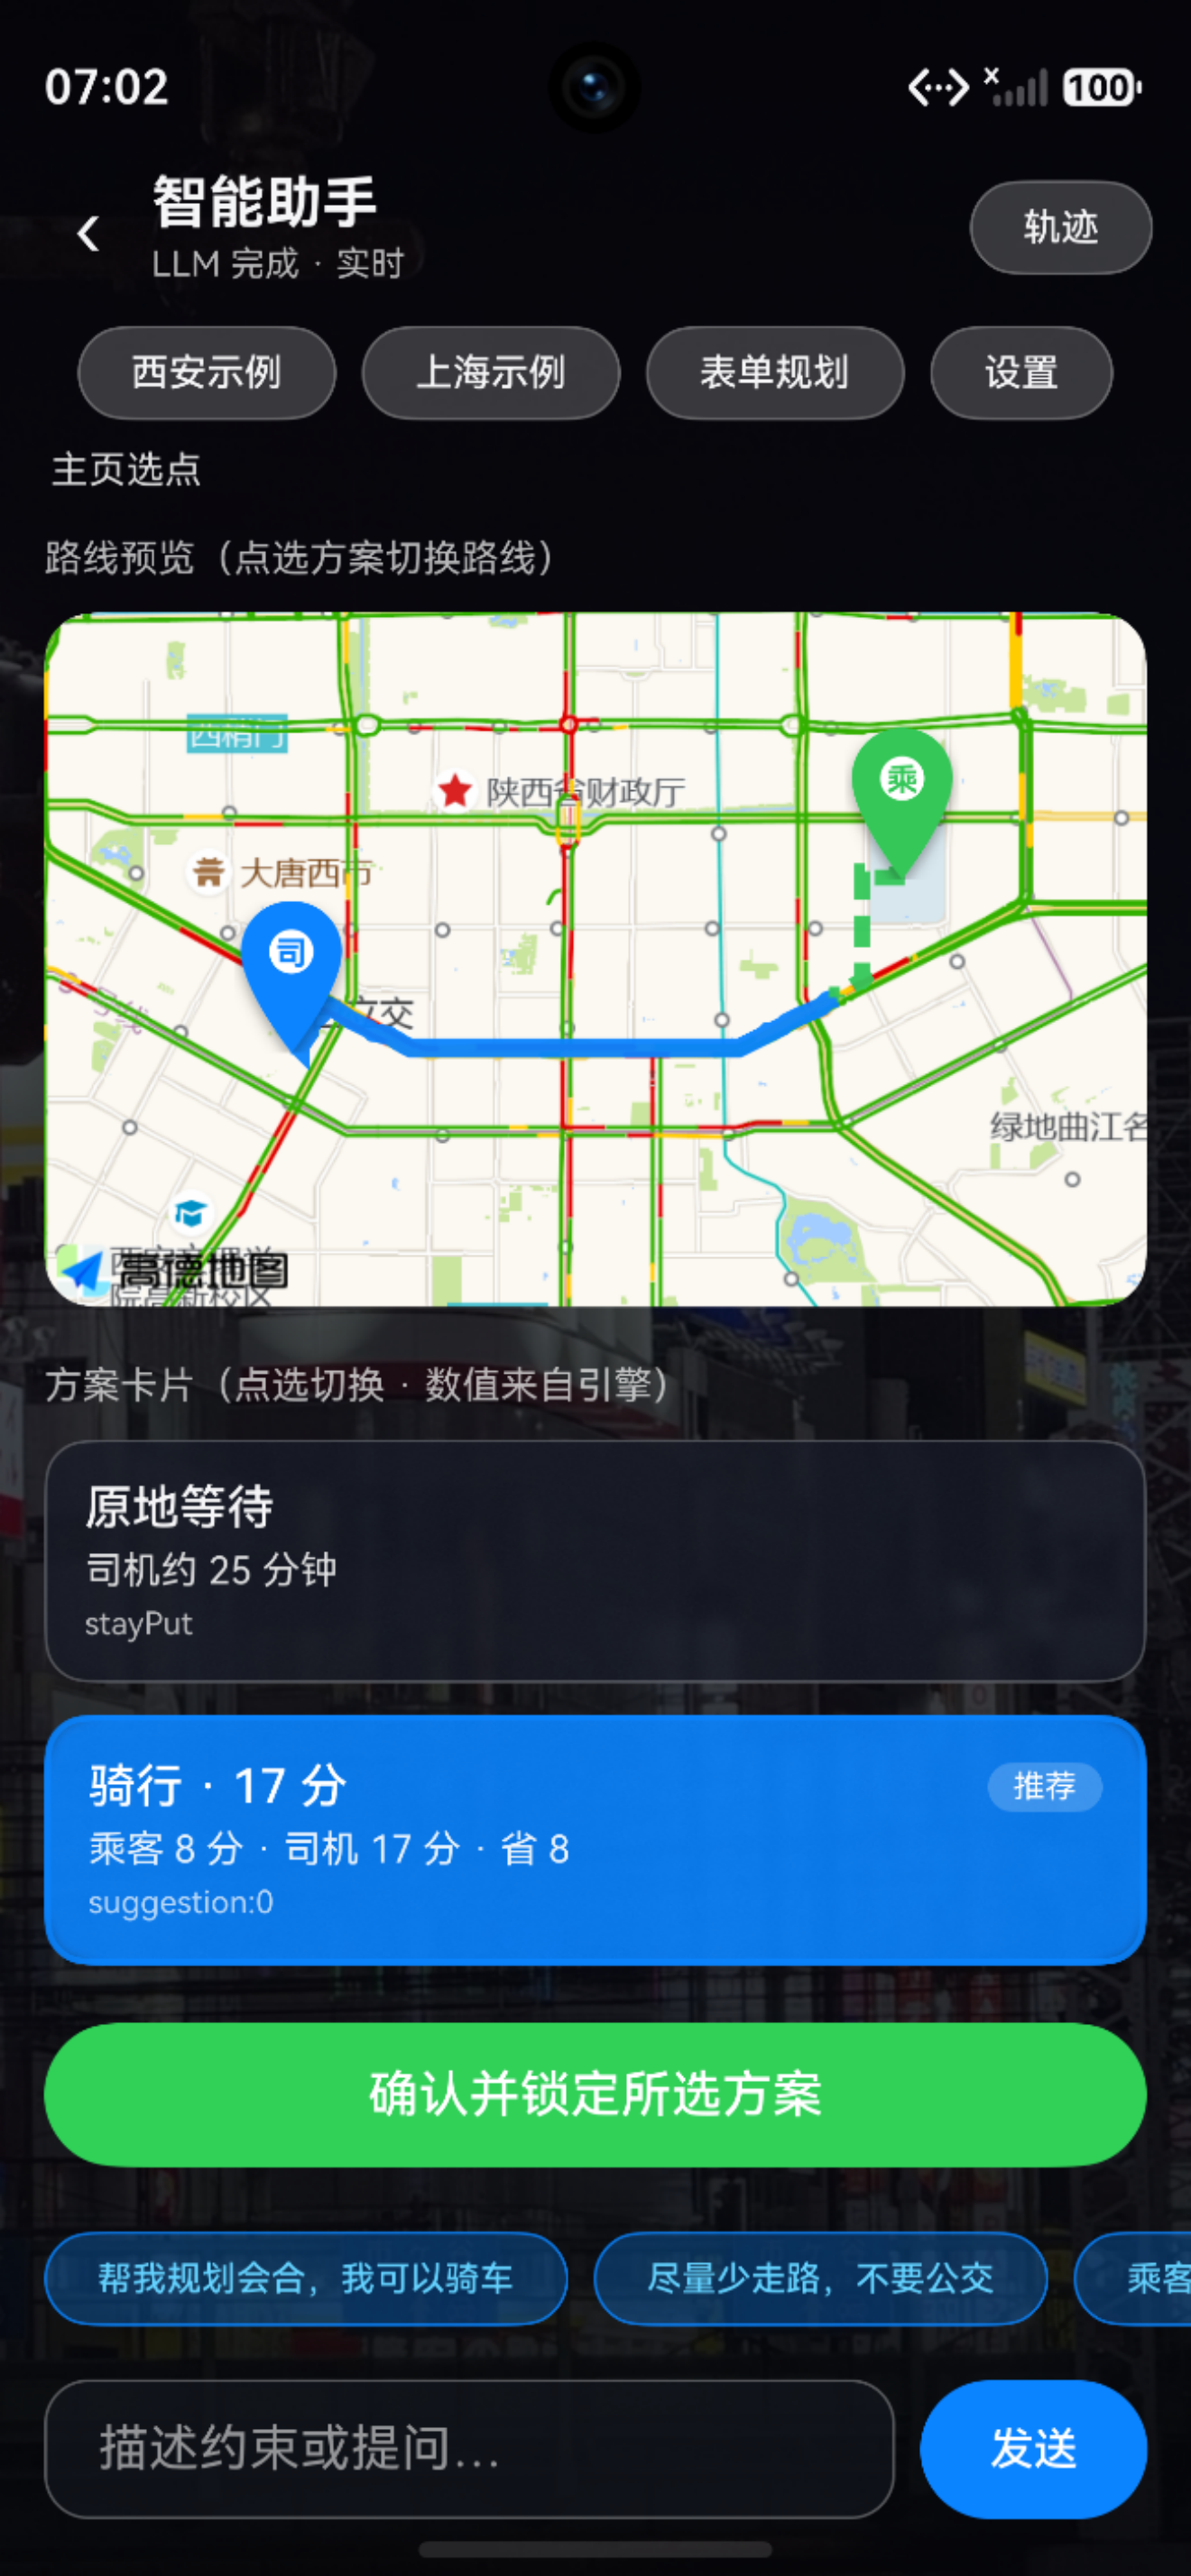
\includegraphics[width=\linewidth]{result_agent_2.png}
    \caption{智能助手方案卡片与锁定入口}
    \label{fig:ui-agent2}
  \end{subfigure}\hfill
  \begin{subfigure}{0.48\textwidth}
    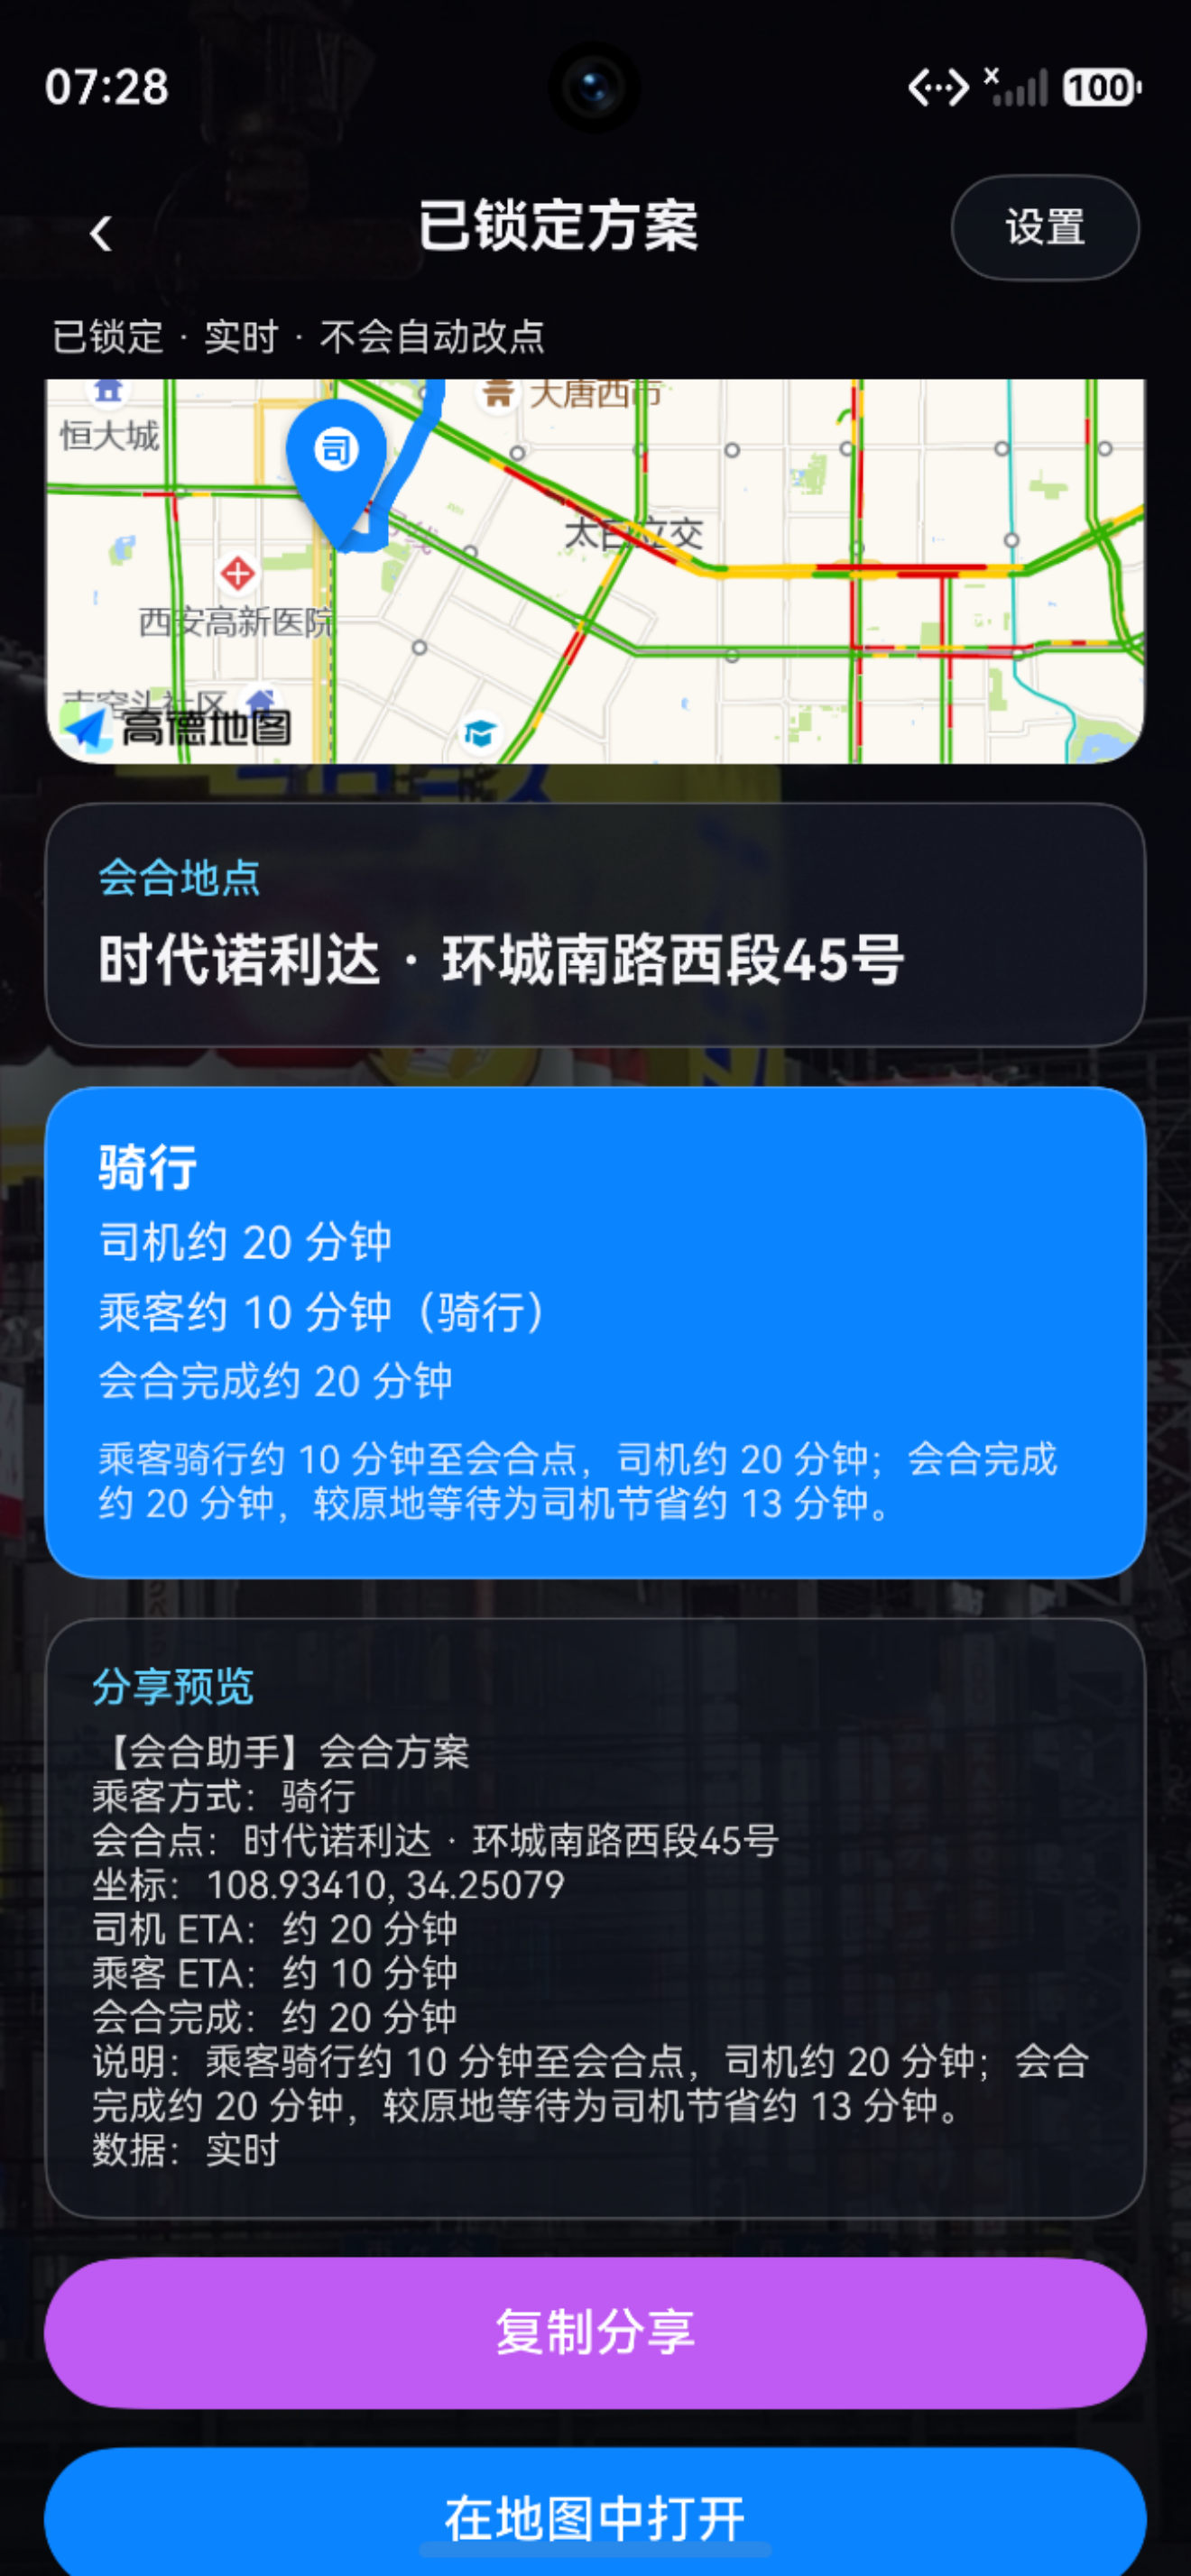
\includegraphics[width=\linewidth]{locked_plan.png}
    \caption{已锁定方案：路线快照 + 分享/导航}
    \label{fig:ui-locked}
  \end{subfigure}
  \caption{方案确认与锁定执行}
\end{figure}

\subsection{界面信息架构}

\begin{table}[H]
\centering
\zihao{5}
\begin{tabularx}{\textwidth}{>{\bfseries}p{2.5cm}X}
\toprule
界面 & 职责 \\
\midrule
主页 & 高德 JS 底图 + 路况；搜索/点选；司机/乘客模式；进入普通规划或智能助手 \\
普通规划 & 草稿起终点只读；乘客方式与步行上限；结果地图与卡片；会合 POI；锁定 \\
智能助手 & 自然语言约束；工具轨迹；路线预览随卡片切换；锁定/分享/打开地图 \\
锁定会话 & 冻结快照；复制分享；系统地图导航；显式重新规划 \\
设置 & Map Web Key、演示 Fixture、LLM Key/Proxy \\
\bottomrule
\end{tabularx}
\caption{主要界面与职责}
\label{tab:screens}
\end{table}

\subsection{系统架构（技术方案）}

\begin{figure}[H]
\centering
\begin{tikzpicture}[
  font=\zihao{5}\songti,
  layer/.style={draw=maDark!60, rounded corners=4pt, align=center,
    inner sep=6pt, fill=white, minimum height=1.05cm},
  mid/.style={layer, text width=5.2cm, minimum width=5.4cm, minimum height=1.55cm},
  arr/.style={-{Latex}, thick, maGray}
]
  \node[layer, minimum width=12.2cm, fill=maSoft] (ui)
    {\textbf{ArkUI 界面层}\\主页地图 · 普通规划 · 智能助手 · 锁定会话};
  \node[layer, minimum width=12.2cm, below=0.55cm of ui, fill=blue!6]
    (agent) {\textbf{Agent 编排}\\工具循环 · 接地校验 · Mode A/B/C};

  % Mid row: leave explicit gap under Agent and above MapProvider
  \node[mid, below left=0.85cm and 0.35cm of agent.south, fill=green!6]
    (tools) {\textbf{工具主机}\\驾车/步行/骑行/公交\\候选 · 评分 · regeo};
  \node[mid, below right=0.85cm and 0.35cm of agent.south, fill=orange!8]
    (engine) {\textbf{本地引擎 domain/}\\路径拦截 · 多模式评分};

  % Anchor bottom layer to the mid-row so boxes never collide
  \node[layer, minimum width=12.2cm, below=0.85cm of $(tools.south)!0.5!(engine.south)$, fill=maSoft]
    (map) {\textbf{Hybrid MapProvider}\\实时 AMap REST/JS · 估算回退 · 诚实 dataSource};

  \draw[arr] (ui) -- (agent);
  \draw[arr] (agent.south) -- ++(0,-0.25) -| (tools.north);
  \draw[arr] (agent.south) -- ++(0,-0.25) -| (engine.north);
  \draw[arr] (tools.south) -- ++(0,-0.30) -| (map.north west);
  \draw[arr] (engine.south) -- ++(0,-0.30) -| (map.north east);
\end{tikzpicture}
\caption{MeetAgent 系统架构}
\label{fig:arch}
\end{figure}

\subsection{Agent 工具与数字接地}

\textbf{硬规则：}界面分钟数、折线、坐标只能源自工具/引擎。防止LLM自行发明路线。

\begin{table}[H]
\centering
\zihao{5}
\begin{tabularx}{\textwidth}{>{\ttfamily}p{3.3cm}X}
\toprule
\normalfont\bfseries 工具 & \bfseries 作用 \\
\midrule
get\_driving\_route & 司机驾车时长、距离、折线（GCJ-02） \\
get\_passenger\_path & 乘客步行/骑行/公交；失败诚实回退估算 \\
generate\_candidates & 沿司机路径生成会合候选 \\
score\_options & 完成时间、司机节省、步行上限等排序 \\
reverse\_geocode / search\_poi & 地点命名与搜索；禁止捏造坐标 \\
parse\_intent（LLM） & 自然语言 $\rightarrow$ 约束；不输出 ETA \\
\bottomrule
\end{tabularx}
\caption{工具边界}
\label{tab:tools}
\end{table}

\subsection{Hybrid 地图与数据源}

\begin{itemize}
  \item \textbf{实时：}Map Web Key + 关闭演示 Fixture——实战接人、看路况。
  \item \textbf{估算：}无 Key 或 Fixture 开启——弱网保底。
  \item \textbf{实时+估算：}部分模式失败回退。
\end{itemize}

对候选会合点 $m$ 与乘客模式 $\mu$，引擎近似优化：
\begin{equation*}
  T_{\mathrm{complete}}(m,\mu)=\max\bigl(T_{\mathrm{driver}}(m),\,T_{\mathrm{passenger}}(m,\mu)\bigr)
\end{equation*}
并相对“原地等待”给出司机节省时间，卡片直接展示这些可解释字段。

\subsection{技术栈}

\begin{table}[H]
\centering
\zihao{5}
\begin{tabularx}{\textwidth}{p{3.0cm}X}
\toprule
\textbf{层次} & \textbf{选型} \\
\midrule
OS / UI & HarmonyOS · ArkTS / ArkUI \\
引擎 & TypeScript \texttt{domain/} + ArkTS 镜像（\texttt{npm test} 25 通过） \\
地图 & Hybrid：Estimate + 高德 Web REST / JS 底图与路况 \\
LLM & OpenAI 兼容（用户 Key / Proxy / Offline） \\
状态 & \texttt{TripDraftStore} 草稿；\texttt{TripSessionStore} 锁定 \\
\bottomrule
\end{tabularx}
\caption{技术栈}
\label{tab:stack}
\end{table}

\subsection{宣传语}

\begin{center}
\fbox{\parbox{0.88\textwidth}{\centering\zihao{4}\songti
\vspace{0.45em}
\textbf{MeetAgent · 会合助手}\\[0.3em]
{\zihao{5} 乘客动一点，司机少绕一点——双方更快见面。}\\[0.15em]
{\zihao{5} HarmonyOS 原生 · 可离线演示 · 确认即锁定}\\[0.45em]
}}
\end{center}

% =============================================================================
\section{介绍文档}
% =============================================================================

{\zihao{5}\songti
% 介绍文档正文（模板要求不超过 800 字）
现实中的接人基本都是“导航到一个固定点就结束”。网约车司机按软件去接乘客，如果乘客周围发生了严重拥堵，网约车会白白浪费十几二十分钟堵在家门口，而乘客只需要走5分钟就可以直接上车；家人去机场接人，出站口人潮里空等半小时；校园或园区里，司机进不了内门，乘客其实骑行几分钟就能到更合适的路口。固定上车点把路况变化和乘客可移动能力都浪费了，双方反复电话改点，体验差、也耗油耗时。

MeetAgent（会合助手）把这类问题收敛成出发前的一次联合规划。用户在鸿蒙手机主页打开实时地图，搜索或点选地点，再确认是乘客位置还是司机出发地；系统用附近兴趣点名称展示地点。随后既可以进入“普通规划”，勾选乘客能否步行、骑行、坐公交并设定步行上限后一键优化；也可以打开“智能助手”，用自然语言说“别走太远、不要公交、我可以骑车”。Hybrid 地图层在配置高德 Key 时拉取实时驾车与乘客路径，失败则回退估算，并标明数据来源。本地引擎沿司机路径生成会合候选，比较完成时间与司机节省，给出骑行、步行、公交与原地等待等可解释卡片，结果地图随方案切换更新路线。大模型只理解约束和解释取舍，不编造分钟数。确认后锁定方案，可复制分享给对方或打开系统地图导航；无大模型密钥时仍能离线规划，保证弱网和演示可用。

产品适合网约车司机自规划、亲友接送、校园园区与医院接驳等场景，单机即可完成选点、规划、锁定与执行；后续可在坚持“数字接地”的前提下扩展行程中风险提示与双端协同。
}

\vspace{0.4em}

\subsection{场景化收益}

\begin{itemize}
  \item \textbf{时间：}用“乘客短途移动”换“司机少绕行”，缩短双方同时到达时间。
  \item \textbf{沟通：}一张锁定卡片 + 分享文案，减少反复改点。
  \item \textbf{信任：}分钟数可追溯到路线工具；数据源徽章避免“假装实时”。
  \item \textbf{可落地：}鸿蒙原生、单机闭环；离线/Fixture 保演示。
\end{itemize}

\subsection{演示/测试步骤}

\begin{enumerate}
  \item 设置 Map Web Key；网络不稳时打开演示 Fixture。
  \item 主页搜索/点选 $\rightarrow$ 指定乘客与司机 $\rightarrow$ 普通规划。
  \item 开始路线优化：对比卡片，切换观察路线变化。
  \item 确认锁定 $\rightarrow$ 复制分享 / 打开地图。
  \item 如要测试智能 Agent 规划，设置 LLM API Key。
  \item 智能助手自然语言约束（如“最多走 8 分钟，不要公交”）。
\end{enumerate}

\subsection{测试}

\begin{itemize}
  \item 领域层：\texttt{cd domain \&\& npm test}（25 项通过）。
  \item 手工清单：\texttt{tests/MANUAL\_CHECKLIST.md}。
  \item 密钥仅存设备偏好或本地 \texttt{.env}，不入库。
\end{itemize}

\subsection{团队}

\begin{table}[H]
\centering
\zihao{5}
\begin{tabularx}{\textwidth}{p{2.4cm}p{2.4cm}X}
\toprule
\textbf{成员} & \textbf{角色} & \textbf{主要贡献} \\
\midrule
李祥熙 & 负责人 & 产品定义、HarmonyOS 实现、引擎与 Agent、作品说明 \\
\bottomrule
\end{tabularx}
\caption{团队分工}
\label{tab:team}
\end{table}

% =============================================================================
\section{附录}
% =============================================================================

\subsection{参考资料}

\begin{enumerate}
  \item 中国高校计算机大赛—人工智能创意赛（鸿蒙赛道）作品说明文档规范（2026.06）。
  \item HarmonyOS 应用开发文档（ArkTS / ArkUI）。
  \item 高德开放平台 Web 服务 API。
\end{enumerate}

\end{document}
